\documentclass[12pt, spanish]{article}
\usepackage[spanish]{babel}
\selectlanguage{spanish}
\usepackage{natbib}
\usepackage{url}
\usepackage[utf8x]{inputenc}
\usepackage{graphicx}
\graphicspath{{images/}}
\usepackage{parskip}
\usepackage{fancyhdr}
\usepackage{vmargin}

\usepackage{minted}


\usepackage{hyperref}
\usepackage[
    type={CC},
    modifier={by-nc-sa},
    version={4.0},
]{doclicense}

\hypersetup{
    colorlinks=true,
    linkcolor=blue,
    filecolor=magenta,      
    urlcolor=cyan,
}

\usepackage[default]{sourcesanspro}

\setmarginsrb{2 cm}{1 cm}{2 cm}{2 cm}{1 cm}{1.5 cm}{1 cm}{1.5 cm}

\title{Modelos de Computación:\\
Práctica 2. \hspace{0.05cm} }                           
\author{Antonio David Villegas Yeguas}                             
\date{\today}                                           

\renewcommand*\contentsname{hola}

\makeatletter
\let\thetitle\@title
\let\theauthor\@author
\let\thedate\@date
\makeatother

\pagestyle{fancy}
\fancyhf{}
\rhead{\theauthor}
\lhead{\thetitle}
\cfoot{\thepage}

\begin{document}
%%%%%%%%%%%%%%%%%%%%%%%%%%%%%%%%%%%%%%%%%%%%%%%%%%%%%%%%%%%%%%%%%%%%%%%%%%%%%%%%%%%%%%%%%

\begin{titlepage}
    \centering
    \vspace*{0.5 cm}
    
\includegraphics[scale = 0.50]{ugr.png}\\[1.0 cm]
    %\textsc{\LARGE Universidad de Granada}\\[2.0 cm]   
    \textsc{\large 3ºA - A2}\\[0.5 cm]            
    \textsc{\large Grado en Ingeniería Informática}\\[0.5 cm]              
    \rule{\linewidth}{0.2 mm} \\[0.2 cm]
    { \huge \bfseries \thetitle}\\
    \rule{\linewidth}{0.2 mm} \\[1 cm]
    
    \begin{minipage}{0.4\textwidth}
        \begin{flushleft} \large
            \emph{Autor:}\\
            \theauthor
            \end{flushleft}
            \end{minipage}~
            \begin{minipage}{0.4\textwidth}
            \begin{flushright} \large
            \emph{Asignatura: \\
            Modelos de Computación}                   
        \end{flushright}
    \end{minipage}\\[0.5cm]
  
    {\large \thedate}\\[0.5cm]
    {\url{https://github.com/advy99/MC/}}
    {\doclicenseThis}
 	
    \vfill
    
\end{titlepage}

%%%%%%%%%%%%%%%%%%%%%%%%%%%%%%%%%%%%%%%%%%%%%%%%%%%%%%%%%%%%%%%%%%%%%%%%%%%%%%%%%%%%%%%%%

%\tableofcontents
%\pagebreak

%%%%%%%%%%%%%%%%%%%%%%%%%%%%%%%%%%%%%%%%%%%%%%%%%%%%%%%%%%%%%%%%%%%%%%%%%%%%%%%%%%%%%%%%%

\section{Descripción del problema}

En mi caso he diseñado un programa en flex++ capaz de encontrar distintas estructuras comunes en un fichero de programación escrito en C/C++. Mi programa leerá un fichero en C/C++ (pasado por argumento) y realizará lo siguiente:

\begin{itemize}
  \item Contar las ordenes del preprocesador.
  \item Mostrar por pantalla que archivos se están incluyendo y en que linea se realiza dicho include.
  \item Mostrar por pantalla el número de definiciones que se están realizando.
  \item Mostrar los comentarios (tanto de linea como en bloque) que se están realizando mostrando también en que linea se realizan.
  \item Contar el número de paréntesis de apertura y cierre. En caso de que no coincidan en número mostrará una advertencia.
  \item Contar el número de llaves de apertura y cierre. En caso de que no coincidan en número mostrará una advertencia.
  \item Mostrar los errores de paréntesis y llaves en el código.
\end{itemize}



\newpage

\section{Solución del problema usando flex++}

En mi caso he abordado el problema de la siguiente forma:




\subsection{Sección de declaraciones}

\begin{minted}[linenos,tabsize=2,breaklines]{c++}
%option noyywrap
%option yylineno

%{
#include <iostream>
#include <fstream>
#include <vector>
#include <stack>

using namespace std;

ifstream fichero;
int ordenes_preprocesador;
int num_defines;

pair<int, int> contar_parentesis = make_pair(0,0);
pair<int, int> contar_llaves = make_pair(0, 0);

vector<pair<string, int> > includes;
vector<pair<string, int> > comentarios_linea;

vector<pair<string, int> > comentarios_bloque;

stack<char> parentesis_llaves;
vector<int> error_parentesis;

string texto;
%}

%%

\end{minted}


Vemos como en esta sección hemos usado la opción de flex \texttt{noyywrap} ya que únicamente leeremos un fichero, además de la opción \texttt{yylineno} para saber que linea esta analizando en ese momento.

También declaramos el flujo por el que leeremos el fichero, y las distintas variables donde guardaremos y contaremos las instrucciones del preprocesador, las llaves, los paréntesis, etc.

Usaremos una pila para controlar las llaves y paréntesis, si están correctamente colocados.


\subsection{Sección de reglas}

\begin{minted}[linenos,tabsize=2,breaklines]{c++}

^"#"

\end{minted}

En esta regla captaremos todas las lineas que comienzan con una almohadilla, por lo que sumaremos uno a las ordenes del preprocesador.



\begin{minted}[linenos,tabsize=2,breaklines]{c++}

^"#include"\ ?[<"][a-zA-Z.a-zA-Z]*[>"]

\end{minted}

En este regla captaremos las lineas que comienzan por "\#include", seguidas por cero o un espacio, y que tienen una cadena de texto dentro, que será el archivo que incluimos. Almacenaremos el archivo que incluimos junto con la línea en la que está haciendo uso de las funciones YYText() y lineno() respectivamente.

También sumaremos uno al contador de ordenes del preprocesador, ya que el include es una orden del preprocesador.


\begin{minted}[linenos,tabsize=2,breaklines]{c++}


^"#define"

\end{minted}

En este regla captaremos las lineas que comienzan por "\#define". Sumaremos uno al contador de defines, y al contador de ordenes del preprocesador.


\begin{minted}[linenos,tabsize=2,breaklines]{c++}

"//".*	

\end{minted}

En esta orden captaremos los comentarios en linea que encontremos, los almacenaremos (junto en la linea en la que están) con la función YYText() y la función lineno().




\begin{minted}[linenos,tabsize=2,breaklines]{c++}

"/*".*"*/"

\end{minted}

Con esta regla captaremos los comentarios en bloque, aunque estén en una única linea. Los almacenaremos junto en la línea en la que están.


\begin{minted}[linenos,tabsize=2,breaklines]{c++}

("/*")+[^"*/"]*("/*")*[^"*/"]*"*/"

\end{minted}

Con esta regla captaremos los comentarios en bloque, considerando que estén en varias lineas, además de que contengan la apertura de otro comentario dentro. Los almacenaremos junto en la línea en la que están.


\begin{minted}[linenos,tabsize=2,breaklines]{c++}

"("

\end{minted}

En esta regla añadiremos un paréntesis a la pila, para comprobar que los paréntesis son correctos.


\begin{minted}[linenos,tabsize=2,breaklines]{c++}

")" 

\end{minted}

En esta regla le haremos un pop a la pila, aunque comprobaremos distintas condiciones:

\begin{enumerate}
	\item Si la pila esta vacía o el símbolo del tope de la pila no es \"(\": Error, cerramos un paréntesis sin abrir ninguno. Añadimos al vector de errores el número de linea y al texto que sacaremos le añadimos ``ERROR-->''.
	\item Si no se cumple la condición anterior: Eliminamos  el tope de la pila.
\end{enumerate}


\begin{minted}[linenos,tabsize=2,breaklines]{c++}

"{" 

\end{minted}

En esta regla añadiremos una llave a la pila, para comprobar que los paréntesis son correctos.



\begin{minted}[linenos,tabsize=2,breaklines]{c++}

"}"

\end{minted}

En esta regla le haremos un pop a la pila, aunque comprobaremos distintas condiciones:

\begin{enumerate}
	\item Si la pila esta vacía o el símbolo del tope de la pila no es "\{": Error, cerramos una llave sin abrir ninguna. Añadimos al vector de errores el número de linea y al texto que sacaremos le añadimos ``ERROR-->''.
	\item Si no se cumple la condición anterior: Eliminamos  el tope de la pila.
\end{enumerate}


\begin{minted}[linenos,tabsize=2,breaklines]{c++}

.

\end{minted}

Sobrescribimos la regla para cualquier carácter, en lugar de mostrarlo por pantalla lo añade a la variable texto, que la mostraremos por pantalla o la mandaremos a un fichero.


\begin{minted}[linenos,tabsize=2,breaklines]{c++}

\n

\end{minted}

Sobrescribimos la regla para los saltos de linea, en lugar de mostrarlo por pantalla lo añade a la variable texto, que la mostraremos por pantalla o la mandaremos a un fichero.\\


\textbf{Común a todas las reglas:}

En todas las reglas añadimos el propio texto, ya que mostraremos el fichero leído, pero con  ``ERROR-->'' en los lugares donde los paréntesis o llaves sean incorrectos.

\subsection{Sección de procedimientos}

Aquí encontraremos el código en C++ encargado de procesar y sacar por pantalla los datos recogidos.

La parte más interesante la podemos encontrar en este fragmento de código, en el que comprobamos si se nos pasa como parámetro una salida para el archivo leído, pero marcando los errores. La parte de contabilizar la seguimos sacando por pantalla.

\begin{minted}[linenos,tabsize=2,breaklines]{c++}

if (argc == 3){
		fstream salida(argv[2], fstream::out);
		salida << texto;
		salida.close();
} else {
		cout << endl << endl << texto;
}


\end{minted}

Los demás datos leídos simplemente los sacamos por pantalla.


\newpage
\section{Ejemplos de ejecución}

Vamos a ejecutar el programa sobre el archivo \texttt{entrada.cc} adjunto.

\begin{center}
	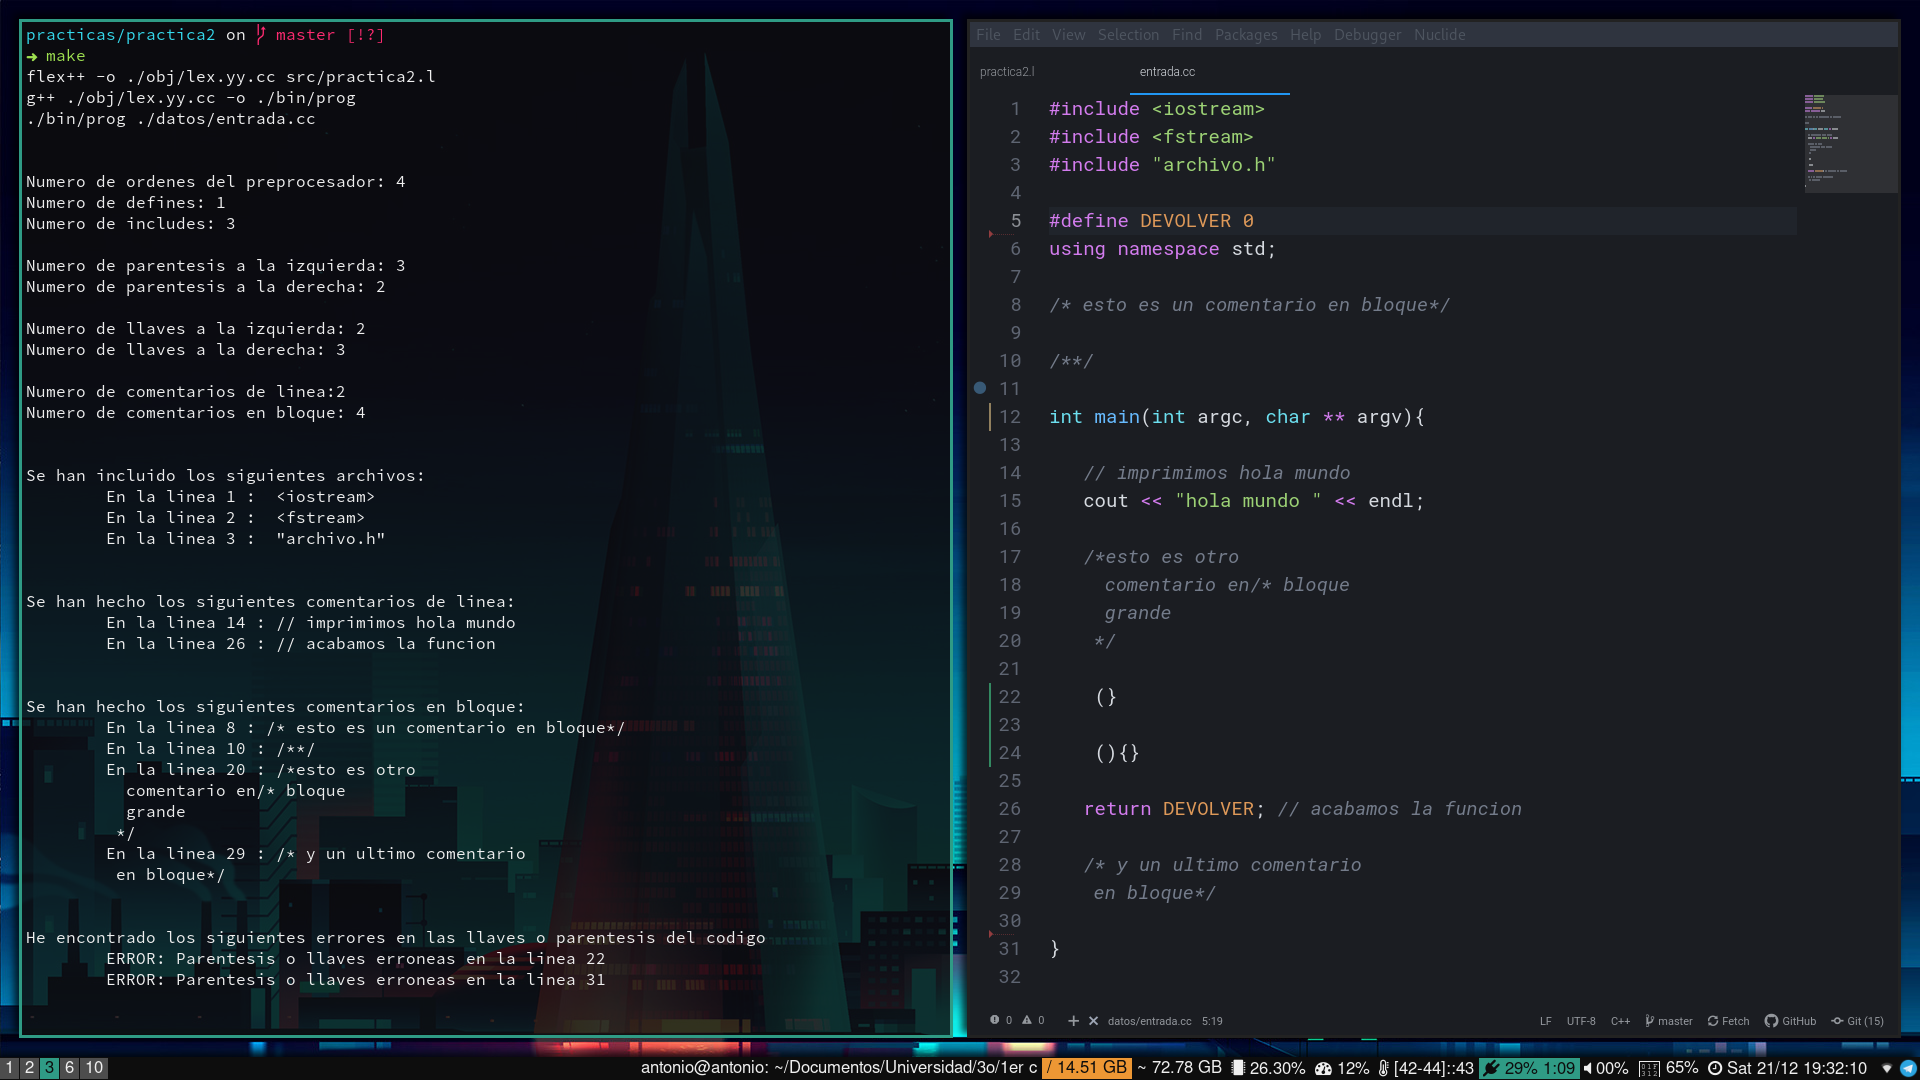
\includegraphics[scale=0.25]{prueba1.png}
\end{center}


Salida de errores en paréntesis y llaves: 

\begin{center}
	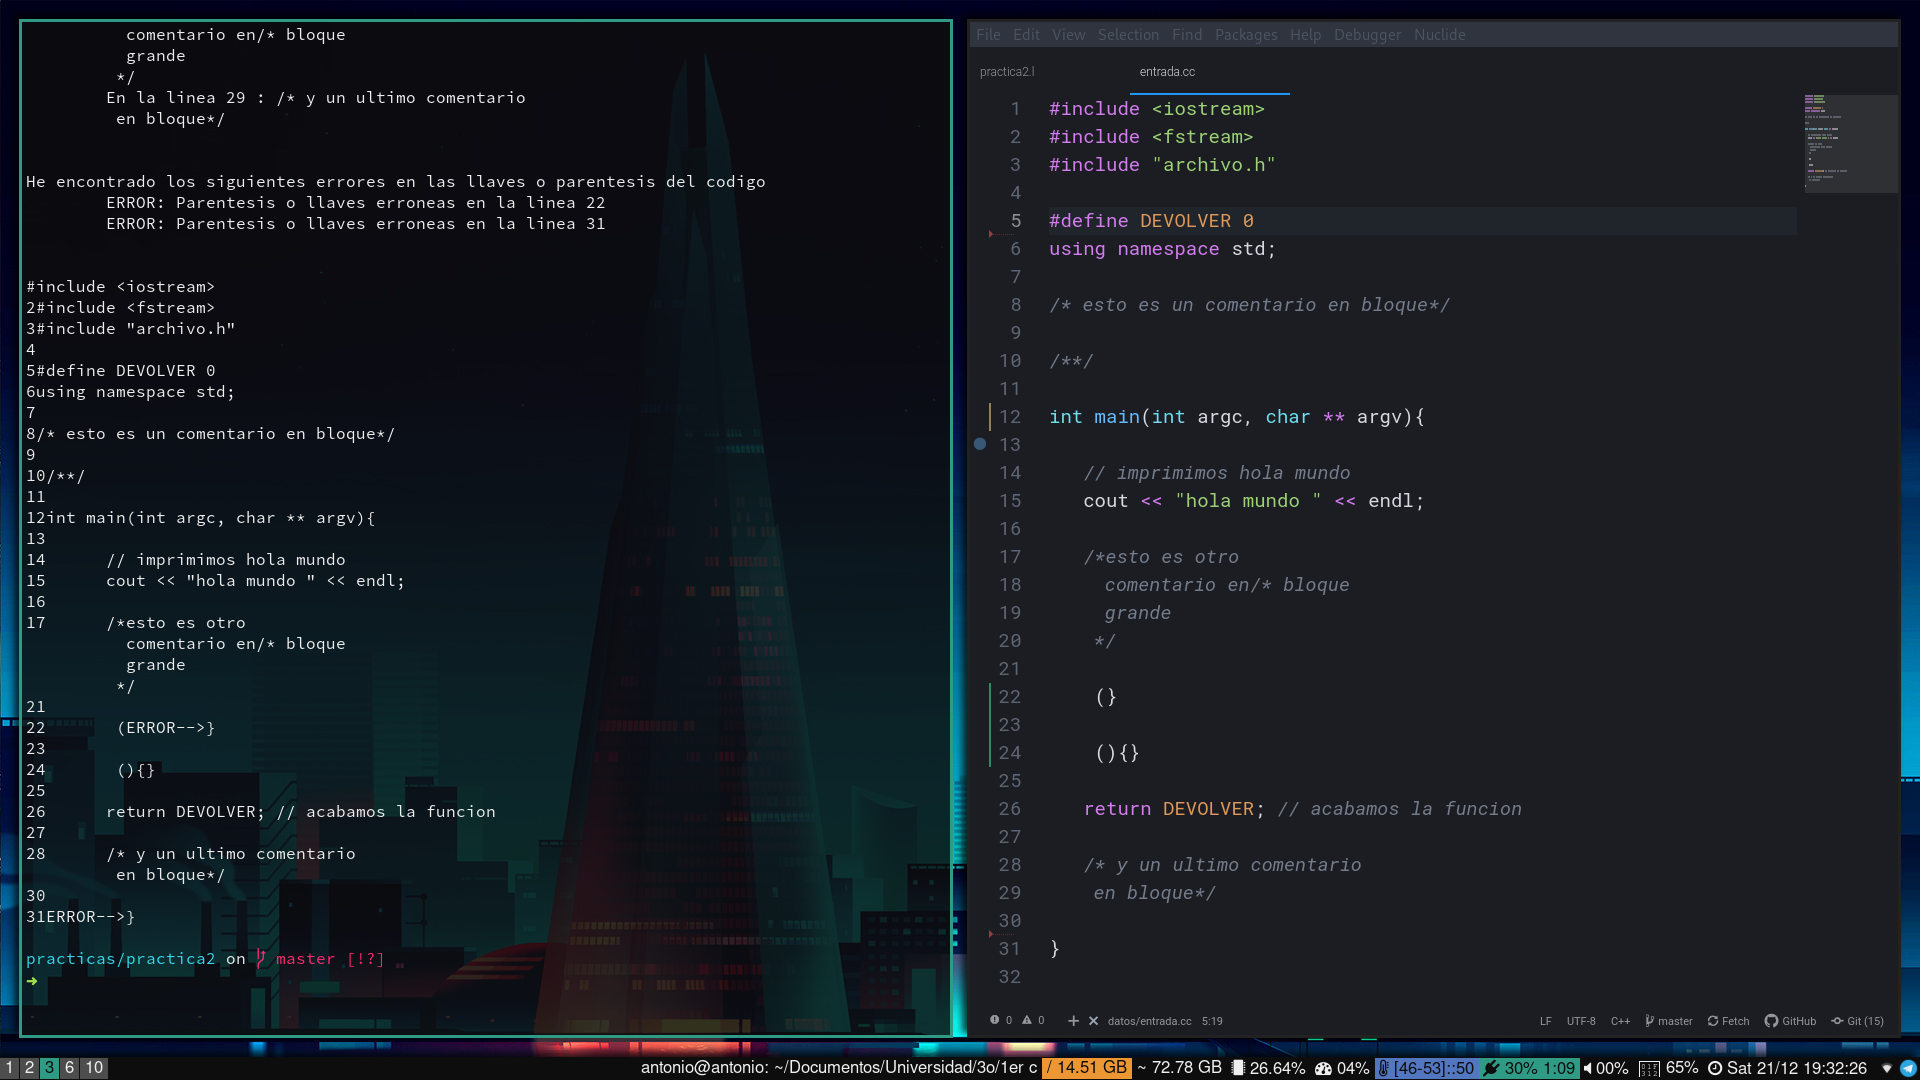
\includegraphics[scale=0.25]{prueba1-2.png}
\end{center}

\newpage

Si le pasamos un parámetro extra la salida marcando los errores irá a ese fichero (si no existe se creará).

\begin{center}
	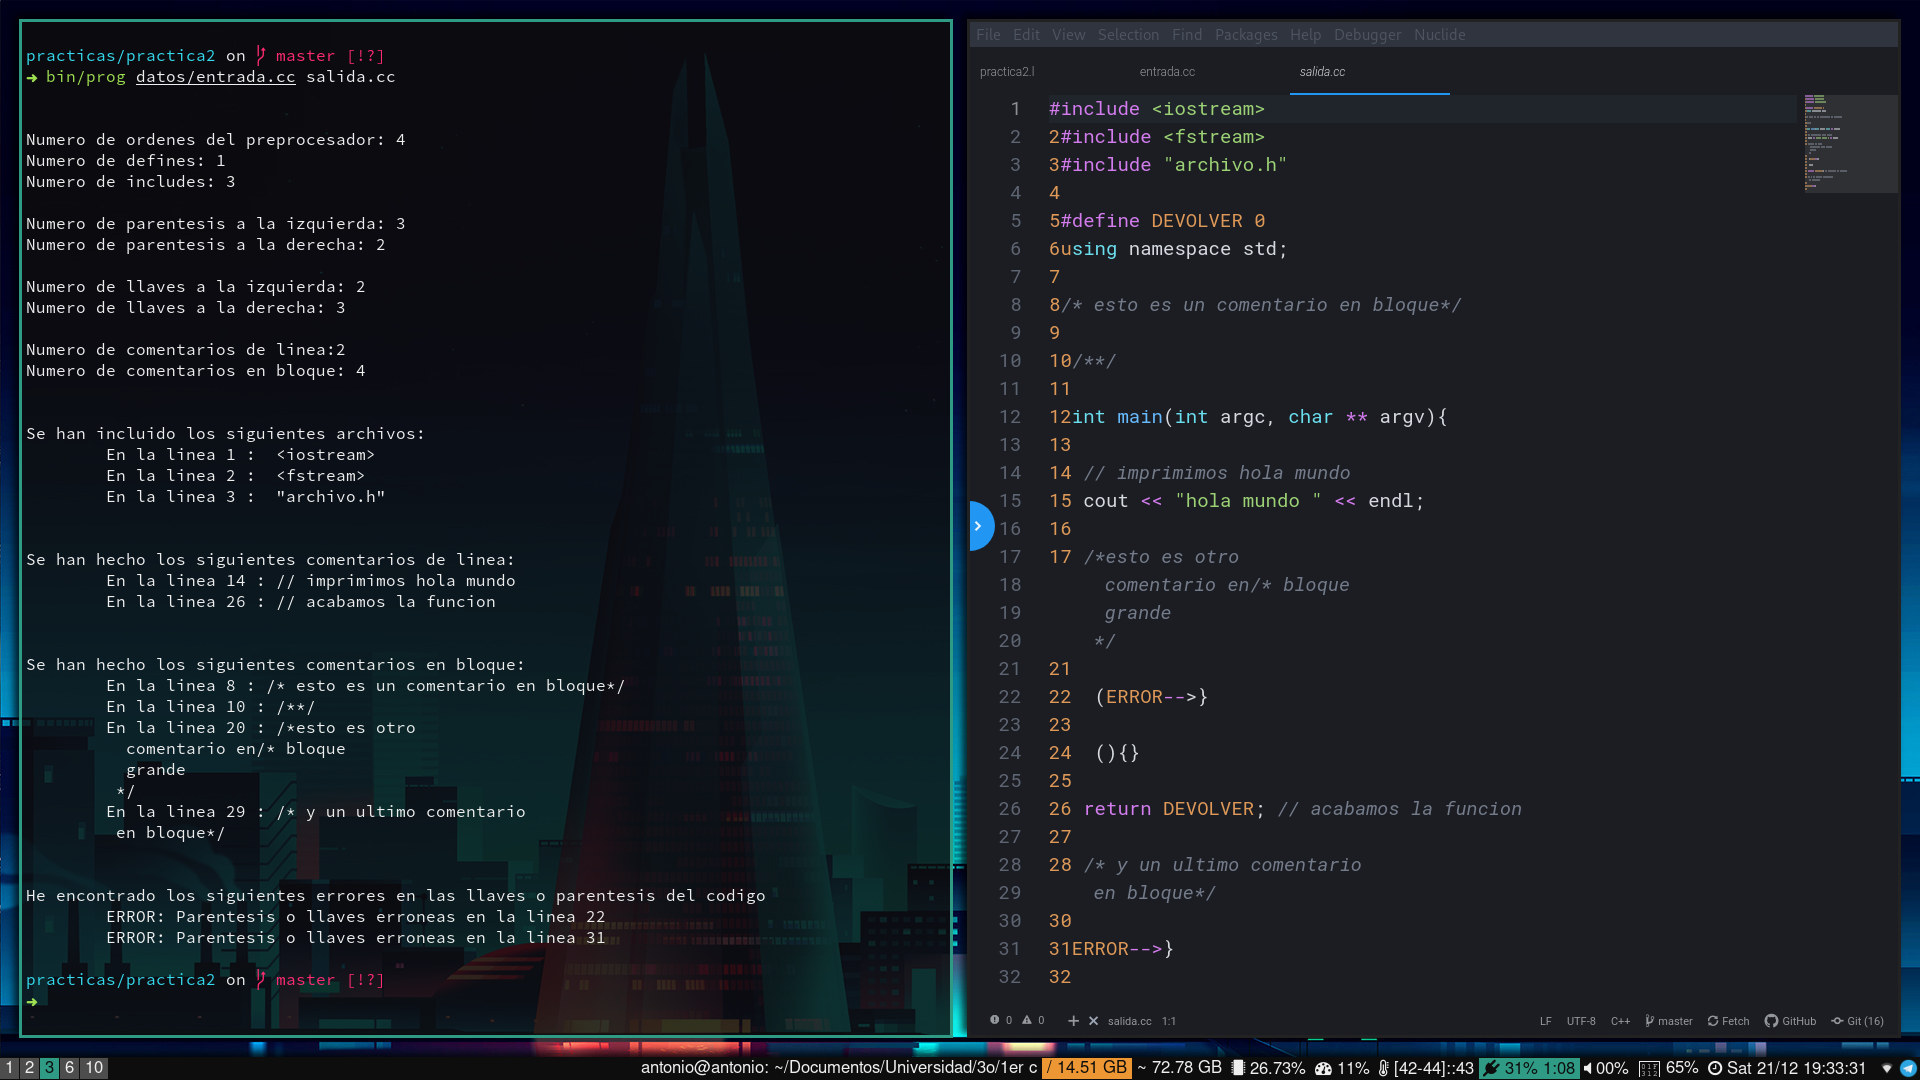
\includegraphics[scale=0.25]{prueba2.png}
\end{center}

\end{document}
